\documentclass[11pt]{article}
\usepackage[utf8]{inputenc}
\usepackage{algorithm}
\usepackage{amsmath}
\usepackage{graphicx}
\usepackage{mathtools}
\usepackage{amsfonts}
\usepackage{hyperref}
\usepackage{geometry}
\usepackage{multicol}
\usepackage{capt-of}
\usepackage{url}
\usepackage{chemmacros}
\usepackage{upgreek}
\usepackage{isomath}
\usepackage{cancel}
\usepackage{bm}
\usepackage[italian]{babel}
\geometry{a4paper, top=2.5cm, bottom=2.5cm, left=3cm, right=3cm, bindingoffset=5mm}
\usepackage[suftesi]{frontespizio}

\title{Esercizi}
\author{Nicolò Favagrossa\\nicolo.favagrossa@studenti.unimi.it, C.M.:969124.}
\date{22 aprile 2024\\A.A. 2023-2024}
\begin{document}
\maketitle
\tableofcontents
\newpage
\section{Esercizio 3.1}
\begin{figure}[htp!]
  \centering
  
\includegraphics[scale=0.3]{Esercizio3.1/Esercizio.jpg} 
\end{figure}
\textbf{A)} Per calcolare la prima quantità che viene chiesta bisogna ricordare che l'attività è definita come:
\begin{equation} \label{N}
    A=\lambda N \quad \Rightarrow N=\frac{A}{\lambda}
\end{equation}
Dove $\lambda$ è la costante di decadimento. L'attività è presente come un dato del problema mentre la costante di decadimento va ricavata come:
\begin{equation}
    \lambda=\frac{1}{\tau}\quad \Rightarrow\quad \lambda=\frac{\ln{2}}{\tau_{1/2}}=\frac{\ln{2}}{1.81\cdot10^{11}\,s}=0.39\cdot10^{-11}\,s^{-1}
\end{equation}
Ritornando all'equazione (\ref{N}) si ricava il numero di atomi contenuti nel campione:
\begin{equation}
    N_{\ch{^{14}C}}=\frac{A}{\lambda}=\frac{0.25\,\mathrm{Bq}}{0.39\cdot10^{-11}\,s^{-1}}=6.4\cdot10^{10}\,\mathrm{atomi}
\end{equation}
Di conseguenza in $1\,\mathrm{g}$ di carbonio naturale ci sono $6.4\cdot10^{10}\,\mathrm{atomi}$ di $\ch{^{14}C}$. Per fare un veloce confronto all'interno di $1\,\mathrm{g}$ di carbonio naturale sono presenti:
\begin{equation}
    N_{\mathrm{C}}=\frac{N_A}{A}\approx\frac{6\cdot10^{23}}{12}=5\cdot10^{22}\,\mathrm{atomi}
\end{equation}
Di conseguenza vediamo che $N_{\ch{^{14}C}}<< N_{\mathrm{C}}$. 

\textbf{B)} Il primo passo è convertire l'attività da $\mathrm{Ci}$ a $\mathrm{Bq}$:
\begin{equation}
    1\,\mathrm{Ci}=3.7\cdot10^{10}\,\mathrm{Bq}\quad \Rightarrow\quad A=0.15\,\mathrm{Bq}
\end{equation}
L'attività al tempo $t$ è:
\begin{equation}
    A(t)=A_0e^{-\lambda t}=A_0e^{-\frac{\ln{2}}{\tau_{1/2}}}
\end{equation}
Invertendo questa relazione è possibile ottenere il tempo $t$:
\begin{equation*}
    t=-\frac{\tau_{1/2}}{\ln{2}}\ln\left({\frac{A(t)}{A_0}}\right)=-\frac{5730\,\mathrm{yr}}{\ln{2}}\left(\frac{0.15}{0.25}\right)=4175\,\mathrm{yr}
\end{equation*}


\textbf{C)} L'incertezza è:
\begin{equation}
    \sigma_t=\frac{\tau_{1/2}}{\ln(2)}\frac{\sigma_A}{A}=\frac{\tau_{1/2}}{\ln(2)}\frac{1}{\sqrt{N}}=\frac{\tau_{1/2}}{\ln(2)}\frac{1}{\sqrt{AT}}=8187\,\mathrm{yr}\frac{1}{0.15\,\mathrm{Bq}3.6\cdot10^{3}\,s}=385\,\mathrm{yr}
\end{equation}
Avendo visto che $\sigma_A/A=1/\sqrt{N}$ e $T$ il tempo di misura. Quindi il risultato finale è:
\begin{equation}
    t=4200\pm400\,\mathrm{yr}
\end{equation}

\newpage
\section{Esercizio 3.2}
\begin{figure}[htp!]
  \centering
  
\includegraphics[scale=0.2]{Esercizio3.2/Esercizio.jpg} 
\end{figure}
Il numero di $\ch{^{238}U}$ e $\ch{^{235}U}$ al tempo $t$:
\begin{equation}
    N_{238}(t)=N_{0,238}e^{-\frac{\ln{2}}{\tau_{1/2}}t} \qquad N_{235}(t)=N_{0,235}e^{-\frac{\ln{2}}{\tau_{1/2}}t}
\end{equation}
Facendo il rapporto tra queste due quantità:
\begin{equation}
    \frac{N_{235}(t)}{N_{238}(t)}=\frac{N_{0,235}}{N_{0,238}}e^{-\ln{2}\left(\frac{1}{\tau_{1/2,235}}-\frac{1}{\tau_{1/2,238}}\right)t}
\end{equation}
Dalle ipotesi dell'esercizio abbiamo che il rapporto di $\ch{^{238}U}$ e $\ch{^{235}U}$ al tempo iniziale sia uguale a $\sim1$. Invece il rapporto al tempo $t$ è $\sim0.007$. Invertendo la relazione si può trovare il valore di $t$.
\begin{equation}
    t=-\frac{\ln\left({\frac{N_{235}(t)}{N_{238}(t)}}\right)}{\ln{2}\left(\frac{1}{\tau_{1/2,235}}-\frac{1}{\tau_{1/2,238}}\right)}=6.1\cdot10^{9}\,\mathrm{yr}
\end{equation}
Possiamo anche stimare "l'incertezza" dell'assunzione fatta: $\frac{N_{0,235}}{N_{0,238}}=2$:
\begin{equation}
    t=-\frac{\ln\left({\frac{N_{235}(t)}{N_{238}(t)}}\right)\pm\ln\left({\frac{N_{0,235}}{N_{0,238}}}\right)}{\ln{2}\left(\frac{1}{\tau_{1/2,235}}-\frac{1}{\tau_{1/2,238}}\right)}=(6.1\pm0.8)\cdot10^{9}\,\mathrm{yr}
\end{equation}
Quindi anche se lasciamo una certa variazione sulle condizioni iniziali troviamo lo stesso ordine di grandezza.
\newpage
\section{Esercizio 4.1}
\begin{figure}[htp!]
  \centering
  
\includegraphics[scale=0.2]{Esercizio4.1/Esercizio.jpg} 
\end{figure}
\textbf{A)} Il primo passo è calcolare il $Q$ valore del decadimento:
\begin{equation}
\begin{array}{c}
      Q=m(\ch{^{224}Ra})-m(\ch{^{220}Rm})-m(\ch{^4He})=\\
     =224\,\mathrm{u}+18.825\,\mathrm{MeV}-220\,\mathrm{u}-10.612\,\mathrm{MeV}-4\mathrm{u}-2.425\,\mathrm{MeV}=5.788\,\mathrm{MeV}
\end{array}
\end{equation}
Ora ricavo il fattore di Gamow dalla relazione della vita media e non dalla formula di $G$ visto che come si è visto si porta un errore di anche due ordini di grandezza:
\begin{equation}
    \ln(\tau)=\ln\left({\sqrt{\frac{m}{2(Q+V_0)}}\frac{a}{2}}\right)+2G
\end{equation}
Per essere consistente con le unità di misura dovrei scrivere:
\begin{equation}
    2G=\ln(\tau)-\ln\left({\sqrt{\frac{m}{2(Q+V_0)}}\frac{a}{2}}\right)=\ln\left({\sqrt{\frac{2(Q+V_0)}{m}}\frac{2\tau}{a}}\right)
\end{equation}
In unità naturali dovrei convertire $\tau$ in una lunghezza:
\begin{equation}
    2G=\ln\left({\sqrt{\frac{2(Q+V_0)}{m}}\frac{2\tau c}{a}}\right)=\ln\left({\sqrt{\frac{2\cdot35.8\,\mathrm{MeV}}{3730\,\mathrm{MeV}}}\frac{2\cdot 1.4\cdot10^{14}\,\mathrm{m}}{7.2\cdot10^{-15}\,\mathrm{m}}}\right)\approx64
\end{equation}
Dove:
\begin{equation}
    \tau c=\frac{\tau_{1/2}}{\ln{2}}=1.4\cdot10^{14}\,\mathrm{m}, \qquad a=1.2\,\mathrm{fm}A^\frac{1}{3}=7.2\cdot10^{-15}\,\mathrm{m}, \qquad V_0\approx30\,\mathrm{MeV}
\end{equation}
E quindi:
\begin{equation}
    G\approx32
\end{equation}
Se avessimo usato la relazione di Gamow per calcolare $G$:
\begin{equation}\label{G}
    G(\text{Gamow})=\alpha\sqrt{\frac{2m}{Q}}Z_\alpha(Z_{Rn}-Z_\alpha)f\left(\frac{a}{b}\right)
\end{equation}
L'unica quantità che manca è la $b$. Per ricavare $b$ basta prendere il potenziale e porlo uguale a $Q$:
\begin{equation}
    V(r)=\alpha Z_\alpha(Z_{Rn}-Z_\alpha)\frac{\hbar c}{r}
\end{equation}
\begin{equation}
    V(b)=Q \quad \Rightarrow \quad b=\frac{\alpha Z_\alpha(Z_{Rn}-Z_\alpha)\hbar c}{Q}=43.3\cdot 10^{-15}\,\mathrm{m} \quad \Rightarrow \quad \frac{a}{b}=0.17
\end{equation}
E il fattore $f$ che dipende da $\frac{a}{b}$:
\begin{equation}
    f\left(\frac{a}{b}\right)=\left[\arccos{\sqrt{\frac{a}{b}}}-\sqrt{\frac{a}{b}-\frac{a^2}{b^2}}\right]=0.78
\end{equation}
Ora che abbiamo tutti gli ingredienti possiamo riprendendere l'equazione (\ref{G}):
\begin{equation}
    G=\alpha\sqrt{\frac{2m}{Q}}Z_\alpha(Z_{Rn}-Z_\alpha)f\left(\frac{a}{b}\right)=34.9
\end{equation}
Quindi ricapitolando:
\begin{equation}
    G_{\text{spe}}=32 \qquad G_{\text{teo}}=35
\end{equation}
Ricordiamo che la vita media è proporzionale a: $\tau\sim e^{2G}$. Sostanzialmente ho che il rapporto tra le due vite medie:
\begin{equation}
    \frac{\tau_{\text{spe}}}{\tau_{\text{Gamow}}}\sim e^{2(G_{\text{spe}}-G_{\text{teo}})}=2.5\cdot10^{-3}
\end{equation}
Quindi quello che avrei calcolato con la teoria di Gamow e qualcosa di circa $3$ ordini di grandezza minore rispetto a quello misurato sperimentalmente.

\textbf{B)} Il primo decadimento è:
\begin{equation}
    \ch{^{224}Ra}\,\to\,\ch{^{212}Pb}+\ch{^{12}C}
\end{equation}
Prima di tutto bisogna calcolare il $Q$ valore del decadimento:
\begin{equation}
\begin{array}{c}
       Q_C=m(\ch{^{224}Ra})-m(\ch{^{212}Pb})-m(\ch{^{14}C})=\\
     =224\,\mathrm{u}+18.825\,\mathrm{MeV}-212\,\mathrm{u}+7.549\,\mathrm{MeV}-12\mathrm{u}=26.37\,\mathrm{MeV}
\end{array}
\end{equation}
Ora se vado a calcolare il rapporto:
\begin{equation}
    \frac{\tau_C}{\tau_\alpha}=\frac{\sqrt{\frac{m_C}{2(Q_C+V_0)}}}{\sqrt{\frac{m_\alpha}{2(Q_\alpha+V_0)}}}\frac{a_C}{a_\alpha}e^{2(G_C-G_\alpha)}=\sqrt{\frac{m_c}{m_\alpha}\frac{Q_\alpha+V_0}{Q_C+V_0}}\frac{a_C}{a_\alpha}e^{2G_\alpha\left(\frac{G_C}{G_\alpha}-1\right)}
\end{equation}
Il primo fattore moltiplicativo:
\begin{equation}\label{t}
    \sqrt{\frac{m_c}{m_\alpha}\frac{Q_\alpha+V_0}{Q_C+V_0}}\frac{a_C}{a_\alpha}=1.38
\end{equation}
Vedo quindi che il fattore puramente cinematico, il rapportorto delle vite medie si porta circa il $40\%$. Significa che il decadimento del carbonio ci "mette" il $40\%$ del tempo in più a decadere (questo solo per il contributo cinematico).
Invece:
\begin{equation}
    \frac{G_C}{G_\alpha}=\frac{\sqrt{\frac{m_C}{Q_C}}}{\sqrt{\frac{m_\alpha}{Q_\alpha}}}\cdot\frac{Z_C(Z_{Rn}-Z_C)}{Z_\alpha(Z_{Rn}-Z_\alpha)}\cdot\frac{f\left(\frac{a}{b}\right)_C}{f\left(\frac{a}{b}\right)_\alpha} = 0.81\cdot2.86\cdot 0.76=1.76
\end{equation}
Il primo e il terzo termine tendono a ridurre il fattore di Gamow. Il secondo termine invece tende ad aumentarlo (il termine che rappresenta l'altezza della barriera di potenziale). Ritornando all'equazione (\ref{t}):
\begin{equation}
     \frac{\tau_C}{\tau_\alpha}=1.8\cdot10^{21}
\end{equation}
Quindi la vita media del decadimento in $\ch{^{12}C}$ è di $21$ ordini di grandezza maggiore rispetto al decadimento in $\alpha$.
\begin{equation}
    \tau_C=1.8\cdot10^{21}\tau_\alpha=7.2\cdot10^{19}\,\mathrm{yr}
\end{equation}
Una cosa importante da capire è che questo decadimento pur essendo poco probabile rispetto al decadimento in $\alpha$ è comunque possibile. Calcolando il $BR$ è possibile quantificare quanti atomi di $\ch{^{224}Ra}$ ho bisogno per vedere un solo decadimento in $\ch{^{12}C}$:
\begin{equation}
    \mathrm{B.R.}=\frac{\lambda_C}{\lambda}=\frac{\lambda_C}{\lambda_\alpha}=\frac{1/\tau_C}{1/\tau_\alpha}=\frac{\tau_\alpha}{\tau_C}=5.6\cdot10^{-22}
\end{equation}
Quindi dati $10^{22}$ atomi, quando saranno tutti decaduti avrò in media 5 atomi decaduti attraverso $\ch{^{12}C}$.

Il secondo decadimento è:
\begin{equation}
    \ch{^{224}Ra}\,\to\,\ch{^{210}Pb}+\ch{^{14}C}
\end{equation}
Con passaggi analoghi si ricava il $Q$ valore:
\begin{equation}
\begin{array}{c}
       Q_C=m(\ch{^{224}Ra})-m(\ch{^{210}Pb})-m(\ch{^{14}C})=\\
     =224\,\mathrm{u}+18.825\,\mathrm{MeV}-210\,\mathrm{u}+14.728\,\mathrm{MeV}-14\mathrm{u}-3.019\,\mathrm{MeV}=30.53\,\mathrm{MeV}
\end{array}
\end{equation}
Calcolando il rapporto tra le vite medie:
\begin{equation}
    \frac{\tau_C}{\tau_\alpha}=\sqrt{\frac{m_c}{m_\alpha}\frac{Q_\alpha+V_0}{Q_C+V_0}}\frac{a_C}{a_\alpha}e^{2G_\alpha\left(\frac{G_C}{G_\alpha}-1\right)}=3.8\cdot10^{33}
\end{equation}
Con:
\begin{equation}
    \frac{G_C}{G_\alpha}=2.10
\end{equation}
Si nota quindi che questo decadimento ha una vita media di $33$ ordini di grandezza in più rispetto alla vita media del decadimento $\alpha$.
\begin{equation}
    \sin{\theta}d\theta=d(\cos{\theta})
\end{equation}
\newpage
\section{Esercizio 5.3}
\begin{figure}[htp!]
  \centering
  
\includegraphics[scale=0.22]{Esercizio5.3/Esercizio.jpg} 
\end{figure}
La richiesta di reattore critico si traduce in:
\begin{equation}
    \nu q = 1
\end{equation}
Dove $\nu$ rappresenta il numero di neutroni prodotti per fissione che è circa: $\nu\approx 2.4\,\mathrm{n}/\mathrm{fiss}$. Il $q$ invece è dato da due fattori:
\begin{equation}
    q=(1-p_{\mathrm{catt}})_{\mathrm{mod}}\frac{\Bar{\sigma}_{\mathrm{fiss}}}{\Bar{\sigma}_{\mathrm{fiss}}+\Bar{\sigma}_{\mathrm{n},\gamma}}
\end{equation}
Noi sabbiamo che $P_{\mathrm{catt}}=0.47$, quindi:
\begin{equation*}
    \frac{\Bar{\sigma}_{\mathrm{fiss}}}{\Bar{\sigma}_{\mathrm{fiss}}+\Bar{\sigma}_{\mathrm{n},\gamma}}=0.79
\end{equation*}
Di conseguenza:
\begin{equation}
    0.21\Bar{\sigma}_{\mathrm{fiss}}=0.79\Bar{\sigma}_{\mathrm{n},\gamma}
\end{equation}
Indichiamo con $\alpha$ la frazione di $\ch{^{235}U}$. Quindi:
\begin{equation}
    0.21\alpha\sigma_{\mathrm{fiss},235}=0.79\left(\alpha\sigma_{\mathrm{n},\gamma,235}+(1-\alpha)\sigma_{\mathrm{n},\gamma,238}\right)
\end{equation}
Raccogliendo $\alpha$:
\begin{equation}
    \alpha=4.5\%
\end{equation}
Ora vogliamo sapere a quale tempo $\alpha(t)=0.045$:
\begin{equation}
   \alpha(t)=0.045=\alpha(0)\frac{e^{-\frac{\ln{2}}{\tau_{1/2,235}}t}}{e^{-\frac{\ln{2}}{\tau_{1/2,238}}t}}
\end{equation}
Invertendo la relazione si ottiene:
\begin{equation}
    t=2.25\cdot10^{9}\,\mathrm{yr}
\end{equation}
\newpage
\section{Esercizio 9.2}
\begin{figure}[htp!]
  \centering
  
\includegraphics[scale=0.22]{Esercizio9.2/Esercizio.jpg} 
\end{figure}
\textbf{A)} Prima di tutto possiamo calcolare la sezione d'urto attraverso la formula data dal problema:
\begin{equation}
    \sigma = \frac{5.6}{\pi}(1.1\cdot10^{-5}\,\mathrm{GeV}^{-2})^21\,\mathrm{MeV}^2(200\,\mathrm{MeV}\,\mathrm{fm})^2\simeq9\cdot10^{-44}\,\mathrm{cm}^2\simeq9\cdot10^{-18}\,\mathrm{fm}^2
\end{equation}
Per calcolare il libero cammino medio invece è necessario calcolare prima la densità di protoni per centimetro cubo:
\begin{equation}
    n=\rho\frac{N_A}{A}Z=2.2\cdot10^{24}\,P/\mathrm{cm}^3
\end{equation}
Ora il libero cammino medio:
\begin{equation}
    \lambda=\frac{1}{n\sigma}=5\cdot10^{18}\,\mathrm{cm}=5\cdot10^{16}\,\mathrm{m}
\end{equation}
Questa distanza è davvero molto grande infatti:
\begin{equation}
    1\,\text{anno luce}=\pi\cdot10^{7}\,\mathrm{s}(3\cdot10^{8}\,\mathrm{m}/\mathrm{s})\simeq9\cdot10^{15}\,\mathrm{m}
\end{equation}
Quindi il libero cammino medio corrisponde a circa $5$ anni luce.

\textbf{B)} Considerando la potenza di un reattore nucleare e considerando l'energia sprigionata in una sola fissione: circa $E_{\mathrm{fiss}}\approx 200\,\mathrm{MeV}/\mathrm{fiss}$ (questo perchè c'è un guadagno di circa $0.9\,\mathrm{MeV}$ per nucleone per i nuclei con $A\ge200$). Se voglio esprimere l'energia nel S.I.
\begin{equation}
    E_{\mathrm{fiss}}\simeq200\,\mathrm{MeV}/\mathrm{fiss}=200\cdot1.6\cdot10^{-13}\,\mathrm{J}/\mathrm{fiss}=3.2\cdot10^{-11}\,\mathrm{J}/\mathrm{fiss}
\end{equation}
Se ora voglio stimare il numero di fissioni al secondo:
\begin{equation}
    \frac{dN_{\mathrm{fiss}}}{dt}=\frac{7\cdot10^{8}\,\mathrm{W}}{3.2\cdot10^{-11}\,\mathrm{J}/\mathrm{fiss}}=2\cdot10^{19}\,\mathrm{fiss}/\mathrm{s}
\end{equation}
Trattandosi di decadimenti $\beta$, l'ordine di grandezza di energia è del $\mathrm{MeV}$.

Il numero di anti-neutrini prodotti per fissione è:
\begin{equation}
    \frac{dN_{\Bar{\nu}}}{dt}=\frac{dN_{\mathrm{fiss}}}{dt}n_{\nu/\mathrm{fiss}}\sim2\cdot10^{19}\,\mathrm{fiss}/\mathrm{s}\cdot 5\nu/\mathrm{fiss}\approx10^{20}\nu/\mathrm{s}
\end{equation}
Dove $n_{\nu/\mathrm{fiss}}$ rappresenta il numero medio di neutrini per fissione. Invece il flusso di neutrini è dato da:
\begin{equation}
    \Phi=\frac{dN_\nu/dt}{4\pi R^2}=\frac{10^{20}\nu/\mathrm{s}}{4\pi 10^6\,\mathrm{cm}^2}=8\cdot10^{12}\,\nu/\mathrm{cm}^2\mathrm{s}
\end{equation}

\textbf{C)} Il numero di interazioni è dato da:
\begin{equation}\label{D}
    \frac{dN_{\text{int}}}{dt}=\Phi N_T\sigma
\end{equation}
Per calcolare la densità di bersagli:
\begin{equation}
    N_T=m\frac{N_A}{A}2=\frac{4}{3}\cdot10^{28}\,\mathrm{protoni}
\end{equation}
E quindi usando l'espressione (\ref{D}) si ricava:
\begin{equation}
    \frac{dN_{\text{int}}}{dt}=\Phi N_T\sigma=8\cdot10^{12}\,\nu/\mathrm{cm}^2\mathrm{s}\cdot\frac{4}{3}\cdot10^{28}\,\mathrm{protoni}\cdot9\cdot10^{-44}\,\mathrm{cm}^2=10^{-2}\,\mathrm{interazioni}/\mathrm{s}
\end{equation}
Anche se la sezione d'urto è estremamente piccola abbiamo la combinazione di un gran numero di neutrini e un gran numero di bersagli mi porta ad avere un tasso di interazione ragionevole. Infatti:
\begin{equation}
    3600\,\mathrm{s}/\mathrm{h}\cdot10^{-2}\,\mathrm{interazioni}/\mathrm{s}=36\,\,\mathrm{interazioni}/\mathrm{h}
\end{equation}
\newpage
\section{Esercizio 10.1}
\begin{figure}[htp!]
  \centering
  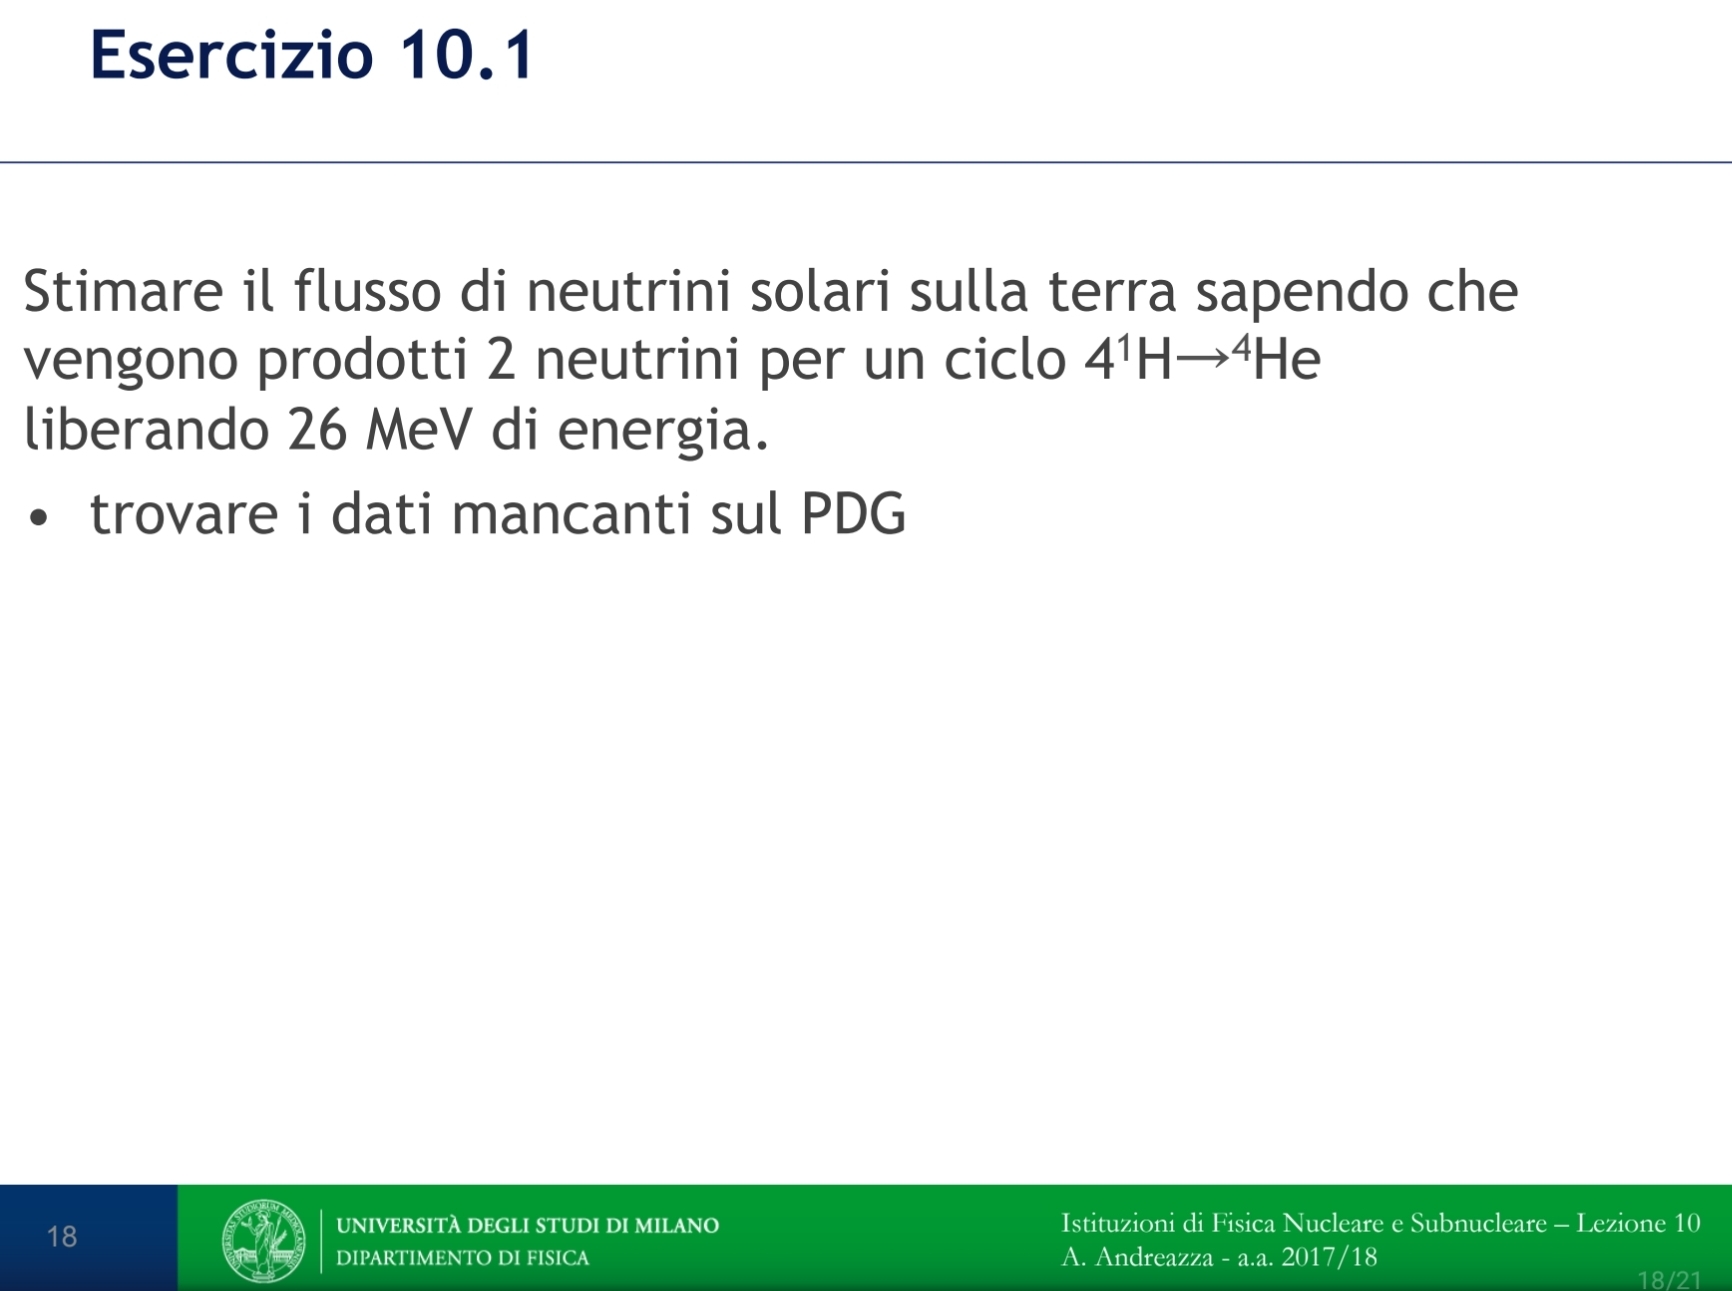
\includegraphics[scale=0.22]{Esercizio10.1/Esercizio.jpg} 
\end{figure}
Prima di tutto bisogna calcolare quanti cicli avvengono al secondo. Per fare questo è necessario conoscere la massa del sole: $M_{\odot}=2\cdot10^{30}\,\mathrm{kg}$ costituiti in massima parte da idrogeno. Grazie a questo è possibile calcolare il numero di atomi di idrogeno:
\begin{equation}
    N_H=M_{\odot}\frac{N_A}{A}=1.2\cdot10^{57}
\end{equation}
Conoscendo anche la potenza irraggiata dal sole: $L_\odot=4\cdot10^{26}\,\mathrm{W}$ è possibile calcolare il numero di cicli di fusione al secondo:
\begin{equation}
    \frac{dN_{\mathrm{fusioni}}}{dt}=\frac{L_\odot}{24.68\,\mathrm{MeV}}=10^{38}\,\mathrm{s}^{-1}
\end{equation}
Dove $24.68\,\mathrm{MeV}$ è l'energia liberata dopo un solo ciclo di fusione. Ogni ciclo di fusione produce $2$ netrini e quindi:
\begin{equation}
    \frac{dN_\nu}{dt}=2\cdot10^{38}\,\mathrm{s}^{-1}
\end{equation}
Il flusso dei neutrini si calcola:
\begin{equation}
    \Phi=\frac{dN_{\nu}/dt}{4\pi R^2}=8\cdot10^{10}\,\nu/\mathrm{cm}^2\mathrm{s}
\end{equation}
Dove $R=1.5\cdot10^{11}\,\mathrm{m}$ è la distanza della terra rispetto al sole.
\newpage
\section{Esercizio 13.1}
\begin{figure}[htp!]
  \centering
  
\includegraphics[scale=0.22]{Esercizio13.1/Esercizio.jpg} 
\end{figure}
Utilizzando la distribuzione di corpo nero e ricordando la legge di Wien è possibile calcolare l'energia tipica dei fotoni a questa temperatura:
\begin{equation}
    \lambda_{\mathrm{max}}=\frac{b}{T}\quad \Rightarrow\quad E=h\nu=h\frac{c}{\lambda}=\frac{h c T}{b}=1.15\cdot10^{-3}\,\mathrm{eV}
\end{equation}
Successivamente l'energia disponibile nel centro di massa si calcola:
\begin{equation}
    S=\left(\mathbf{P}_p+\mathbf{P}_\gamma\right)^2=m_p^2+0+2E_pE_\gamma-2|\mathbf{p}_p|E_\gamma\cos{\theta}
\end{equation}
Per calcolare l'energia di soglia si calcola il caso in cui $S$ è massimo e quindi:
\begin{equation}
    S_\mathrm{max}: \quad \cos{\theta}=-1
\end{equation}
Di conseguenza l'espressione diventa:
\begin{equation}
    S_\mathrm{max}=m_p^2+2E_pE_\gamma+2|\mathbf{p}_p|E_\gamma
\end{equation}
Ora è possibile porre il protone come ultrarelativistico per semplificare i conti. Successivamente dopo aver controllato il risultato è possibile verificare se questo è vero oppure no. Quindi $|\mathbf{p}_p|\sim E_p$ ($E_p>>m_p$):
\begin{equation}
    S_\mathrm{max}=m_p^2+2E_pE_\gamma+2\sqrt{E_p^2-m_p^2}E_\gamma=m_p^2+4E_pE_\gamma=m^2_\Delta
\end{equation}
Sapendo che la massa della $\Delta$ è: $m_\Delta=1232\,\mathrm{MeV}$ posso calcolare l'energia di soglia del protone per indurre la reazione richiesta:
\begin{equation}
    E_p^{th}=\frac{m_\Delta^2-m_p^2}{4E_\gamma}=1.3\cdot10^{20}\,\mathrm{eV}
\end{equation}
Quindi supporre il protone come una particella ultrarelativistica è corretto.
\newpage
\section{Esercizio 13.2}
\begin{figure}[htp!]
  \centering
  
\includegraphics[scale=0.22]{Esercizio13.2/Esercizio.jpg} 
\end{figure}
\textbf{A)} La risonanza $\Delta^+$ ha: $I=\frac{3}{2}$ e $I_3=+\frac{1}{2}$. Attraverso i coefficienti di Clebsch-Gordan è possibile andare a vedere in che stati può essere. Sicuramente sto facendo la composizione di $1\times1/2$ in quanto abbiamo un pione e un nucleone nello stato finale. Infatti ricordo che $N$ (nucleone) ha: $I=\frac{1}{2}$ e $I_3=\pm\frac{1}{2}$. Mentre il pione ha: $I=1$ e $I_3=\pm1,0$. Vedo che lo stato lo trovo in una combinazione di:
\begin{equation}
    \sqrt{\frac{1}{3}}|\pi^+n\rangle+\sqrt{\frac{2}{3}}|\pi^0p\rangle
\end{equation}
Il $BR$ è proporzionale all'elemento di matrice al quadrato quindi:
\begin{equation}
    \frac{\mathrm{BR}(\Delta^+\,\to\,\pi^+n)}{\mathrm{BR}(\Delta^+\,\to\,\pi^0p)}=\frac{1}{2}
\end{equation}
Quindi il decadimento in $\pi^+n$ avverà la metà delle volte rispetto al decadimento $\pi^0p$

\textbf{B)} Procedendo allo stesso modo si trova che $\Delta^0$ ha: $I=\frac{3}{2}$ e $I_3=-\frac{1}{2}$. Facendo riferimento ai coefficienti di Clebsch-Gordan:
\begin{equation}
    \sqrt{\frac{2}{3}}|\pi^0n\rangle+\sqrt{\frac{1}{3}}|\pi^-p\rangle
\end{equation}
E quindi:
\begin{equation}
    \frac{\mathrm{BR}(\Delta^0\,\to\,\pi^0n)}{\mathrm{BR}(\Delta^0\,\to\,\pi^-p)}=2
\end{equation}

\textbf{C)}  Gli stati di risonanza $N$ sono come i nucleoni ma in stato risonante quindi hanno: $I=\frac{1}{2}$ e $I_3=\pm\frac{1}{2}$. Per lo stato $N^+$ trovo che:
\begin{equation}
    \sqrt{\frac{2}{3}}|\pi^+n\rangle-\sqrt{\frac{1}{3}}|\pi^0p\rangle
\end{equation}
Quindi:
\begin{equation}
     \frac{\mathrm{BR}(N^+\,\to\,\pi^+n)}{\mathrm{BR}(N^+\,\to\,\pi^0p)}=2
\end{equation}

\textbf{D)} Per lo stato $N^0$:
\begin{equation}
    \sqrt{\frac{1}{3}}|\pi^0n\rangle-\sqrt{\frac{2}{3}}|\pi^-p\rangle
\end{equation}
Quindi:
\begin{equation}
    \frac{\mathrm{BR}(N^0\,\to\,\pi^0n)}{\mathrm{BR}(N^0\,\to\,\pi^-p)}=\frac{1}{2}
\end{equation}
\newpage
\section{Esercizio 14.1}
\begin{figure}[htp!]
  \centering
  
\includegraphics[scale=0.22]{Esercizio14.1/Esercizio.jpg} 
\end{figure}
Considerando che la densità del platino è: $\rho_{\mathrm{Pt}}=21.4\,\mathrm{g}/\mathrm{cm}^3$ e $Z=78$. Come massa atomica prendo $A=156$ anche se ci sono numerosi isotopi stabili. Un calcolo più rigoroso includerebbe una media pesata. Richiamando la formula empirica di $I$ per grandi $Z$, si trova che $I\sim 10\,\mathrm{eV}\cdot Z=780\,\mathrm{eV}$.
\begin{figure}[htp!]
  \centering
  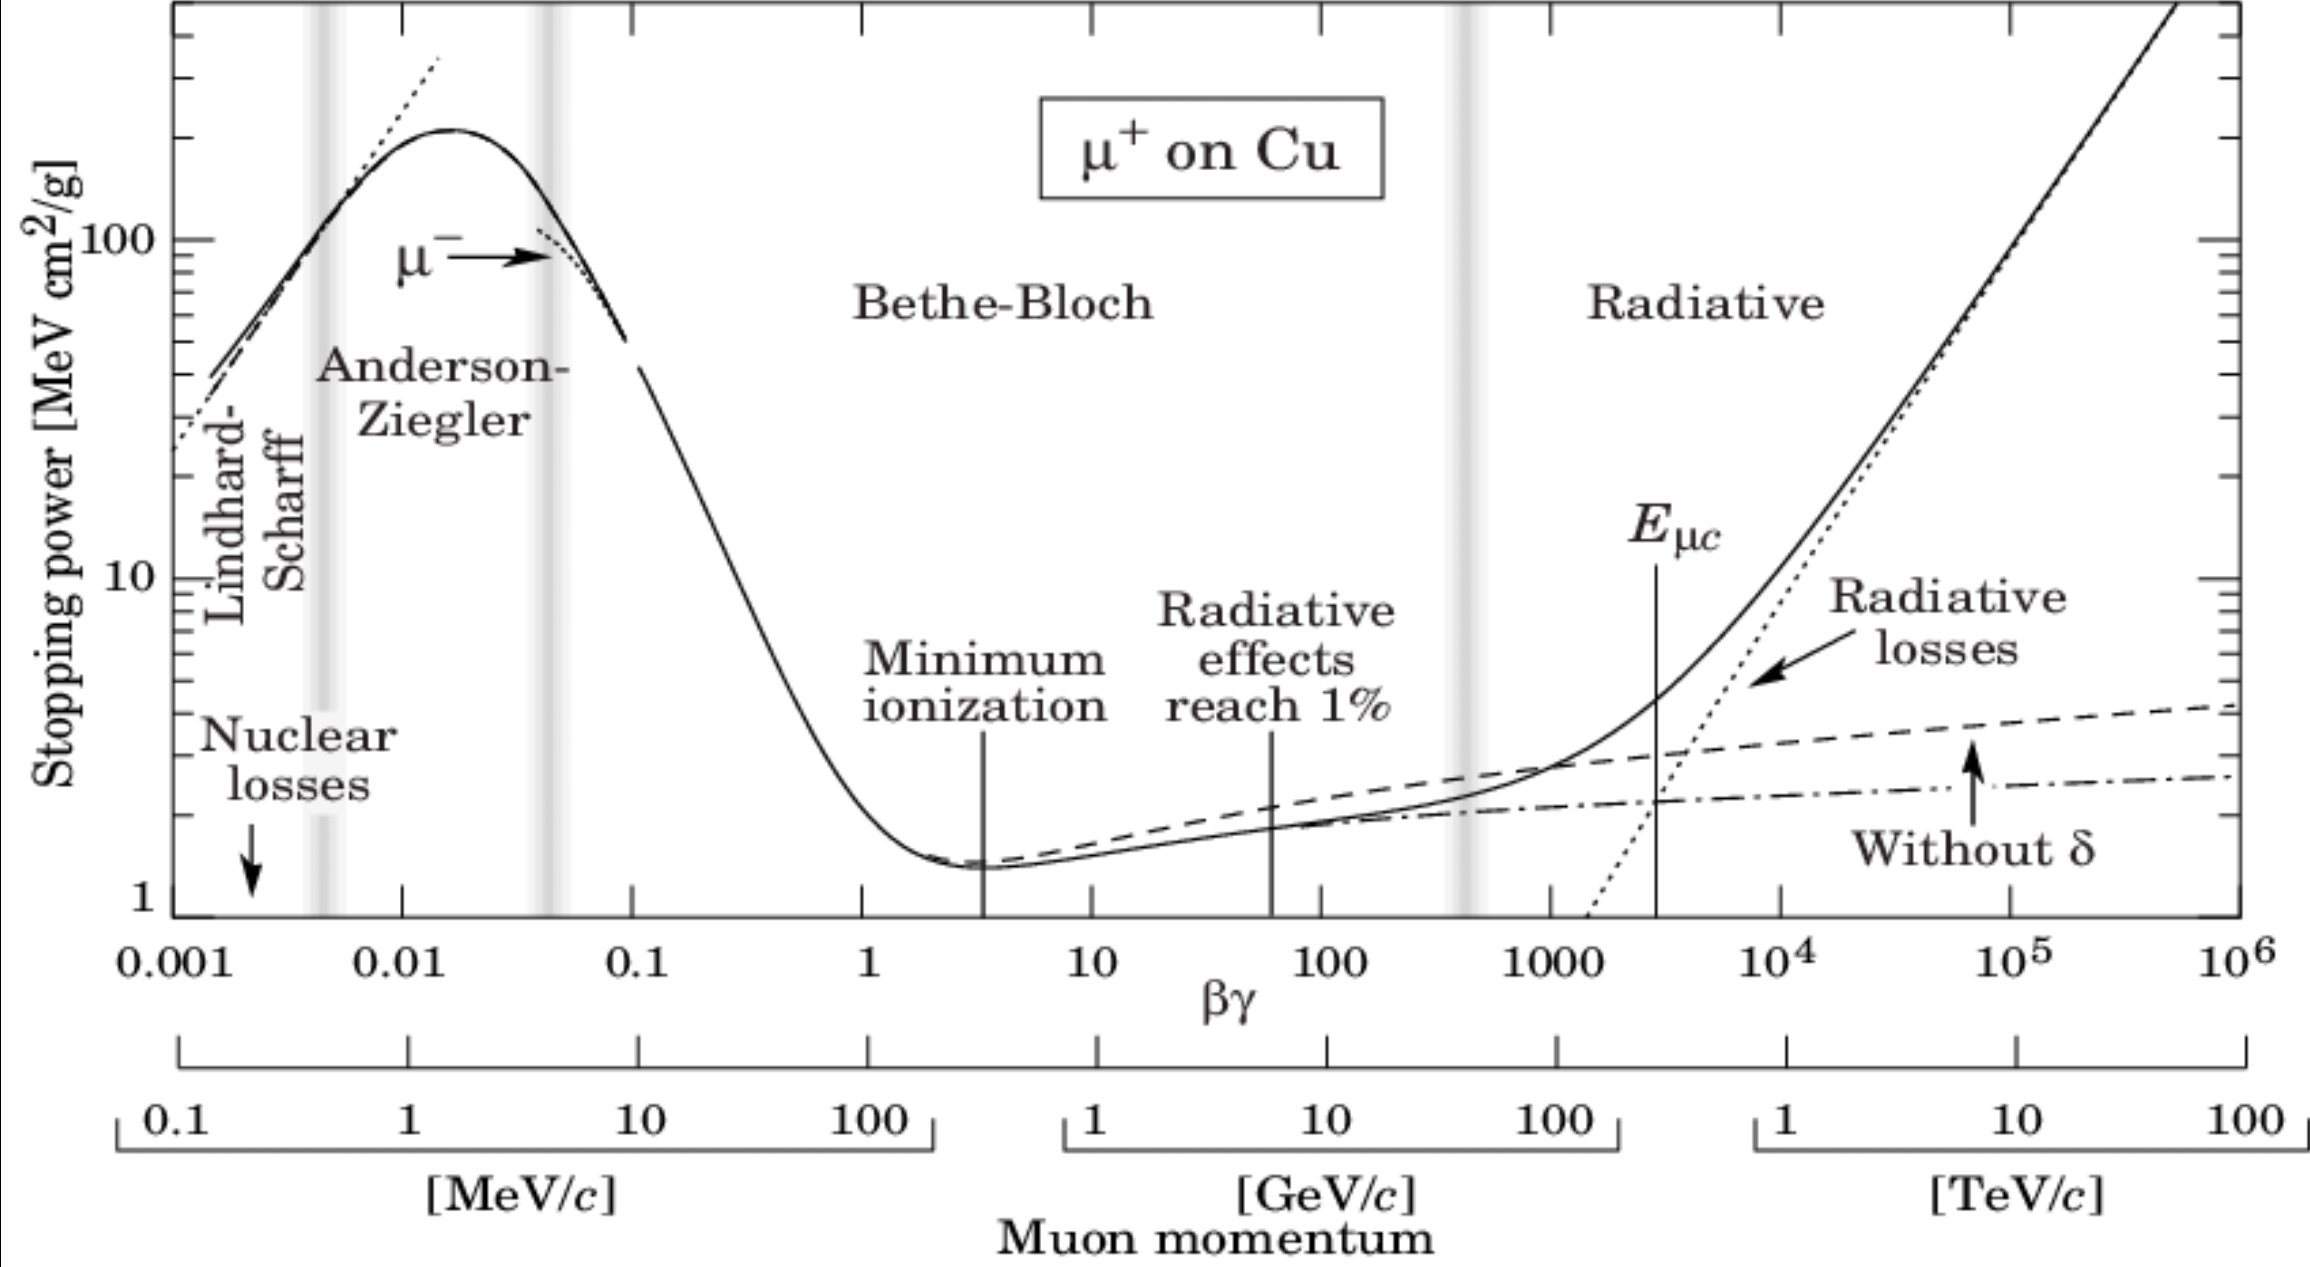
\includegraphics[scale=0.17]{Esercizio14.1/Bethe-Bloch.jpg} 
\end{figure}
Dopo aver calcolato il $\beta\gamma$ per le tre diverse particelle è possibile collocarle all'interno del grafico. Per l'elettrone:
\begin{equation}
    (\beta\gamma)_e=\frac{p}{m_e}\simeq1000
\end{equation}
Quindi siamo a regime ultrarelativistico e quindi possiamo trascurare il contributo della massa all'energi:
\begin{equation}
    E_e=\sqrt{m_e^2+p^2}\simeq p=500\,\mathrm{MeV}
\end{equation}
Per quanto riguarda il muone invece:
\begin{equation}
    (\beta\gamma)_\mu=\frac{p}{m_\mu}\simeq5 
\end{equation}
Sapendo che la massa del muone è: $m_\mu=105\,\mathrm{MeV}$. In questo caso quindi:
\begin{equation}
    E_\mu=\sqrt{m_\mu^2+p^2}=511\,\mathrm{MeV}
\end{equation}
Per il protone:
\begin{equation}
    (\beta\gamma)_p=\frac{p}{m_p}\simeq\frac{1}{2} 
\end{equation}
E quindi l'energia del protone:
\begin{equation}
    E_p\sqrt{m_p^2+p^2}=1063\,\mathrm{MeV}
\end{equation}
Partendo dal muone riconosciamo che si colloca molto vicino al minimo di ionizzazione quindi possiamo approssimare:
\begin{equation}
    \left(\frac{dE}{d(x\rho)}\right)_{\mu}\simeq1.5\,\frac{\mathrm{MeV}}{\mathrm{g}/\mathrm{cm}}
\end{equation}
Moltiplicando per la densità si trova:
\begin{equation}
    \left(\frac{dE}{dx}\right)_{\mu}=32.1\,\mathrm{MeV}/\mathrm{cm}
\end{equation}
Di conseguneza:
\begin{equation}
    \Delta E=-32.1\,\mathrm{MeV}\quad \Rightarrow\quad E_\mu'=479\,\mathrm{MeV} \quad \Rightarrow\quad p_\mu'=\sqrt{E_\mu'^2-m_\mu^2}=467\,\mathrm{MeV}
\end{equation}

Per il protone non si può fare la stessa approssimazione. Scrivendo la formula di Bethe-Bloch:
\begin{equation}
     \left(\frac{dE}{d(x\rho)}\right)_p=4 \pi r_e^2 m_e c^2 N_A\frac{Z}{A}\frac{z^2}{\beta^2}\left[\frac{1}{2} \ln \frac{2 \gamma^2 \beta^2 m_e c^2 T_{\max }}{\bar{I}^2}-\beta^2-\frac{\delta(\gamma \beta)}{2}\right] 
\end{equation}
Le correzioni dovute dalla $\delta$ sono piccole quindi possiamo trascurarlo. Ricordando che:
\begin{equation}
    T_\mathrm{max}=\frac{2\gamma^2\beta^2m_ec^2}{1+2\gamma m_e/M+(m_e/M)^2}\sim2\gamma^2\beta^2m_ec^2
\end{equation}
Con $M>>m_e$. Quindi si semplifica in:
\begin{equation}
    \left(\frac{dE}{d(x\rho)}\right)_p=4 \pi r_e^2 m_e c^2 N_A\frac{Z}{A}\frac{z^2}{\beta^2}\left[ \ln \frac{2\gamma^2\beta^2m_ec^2}{\bar{I}}-\beta^2\right]
\end{equation}
Sostituendo tutte le quantità e utilizzando l'approssimazione che mi chiude tutto il prefattore nel numero $0.15\,\frac{\mathrm{MeV}}{\mathrm{g}/\mathrm{cm}^2}$. Quindi:
\begin{equation}
    \left(\frac{dE}{dX}\right)_p=0.15\,\frac{\mathrm{MeV}}{\mathrm{g}/\mathrm{cm}^2}\frac{1}{\beta^2}\left[\ln \frac{2\gamma^2\beta^2m_ec^2}{\bar{I}}-\beta^2\right]=3.33\,\frac{\mathrm{MeV}}{\mathrm{g}/\mathrm{cm}^2}
\end{equation}
Quindi:
\begin{equation}
    \left(\frac{dE}{dx}\right)_p=71.2\,\frac{\mathrm{MeV}}{\mathrm{cm}}
\end{equation}
\begin{equation}
    \Delta E=-71.2\,\mathrm{MeV}\quad \Rightarrow\quad E_p'=992\,\mathrm{MeV} \quad \Rightarrow\quad p_p'=\sqrt{E_p'^2-m_p^2}=323\,\mathrm{MeV}
\end{equation}

Per quanto riguarda l'elettrone invece abbiamo già detto che è una particella a regime ultrarelativistico. La parte radiativa è quindi molto importante. Andando a guardare il sito consigliato dall'esercizio si vede che l'energia critica per il $Pt$ è di $7.59\,\mathrm{MeV}$ per gli elettroni. Significa che se l'energia nel nostro caso è molto maggiore di questa possiamo considerare solo il contributo radiativo, se invece è molto minore possiamo considerare solo il contributo collisionale. Nel caso in cui l'energia in gioco si a comparabile con questa energia critica bisogna considerare entrambi i contributi. Nel nostro caso abbiamo un elettrone di $E_e=500\,\mathrm{MeV}$ e quindi: $E_e>>E_{\text{crit}}$. Possiamo considerare solo termine radiativo. Quindi la perdita di energia è:
\begin{equation}
     \left(\frac{dE}{d(x\rho)}\right)_e=-\frac{E}{X_0}
\end{equation}
Dove:
\begin{equation}
    X_0=\frac{716.4 A}{Z(Z+1)\ln({287/\sqrt{z}})}\,\frac{\mathrm{g}}{\mathrm{cm}^2}=6.5\,\frac{\mathrm{g}}{\mathrm{cm}^2}
\end{equation}
E quindi:
\begin{equation}
    \left(\frac{dE}{dx}\right)_e=1666\,\frac{\mathrm{MeV}}{\mathrm{cm}}
\end{equation}
Verrebbe una $\Delta E=-1666\,\mathrm{MeV}$ che è impossibile. Siamo in una condizione in cui non vale $\frac{dE}{dx}x<<E$ e quindi non si può semplicemente moltiplicare lo spessore per la perdita di energia. Infatti bisogna tenere in considerazione che l'elettrone man mano che perde energia rallenta e quindi cambia anche il modo in cui perde energia. Quindi:
\begin{equation}
    \frac{dE}{E}=\frac{1}{X_0}dx\quad \Rightarrow\quad\int_{E_0}^{E'}\frac{dE}{E}=\frac{1}{X_0}\int_0^xdx
\end{equation}
Trovando come soluzione:
\begin{equation}
    E(x)=E_0e^{-\frac{x}{X_0}} \quad \Rightarrow\quad E(1\,\mathrm{cm})=25\,\mathrm{MeV}>>m_e \quad \Rightarrow\quad p_e'\simeq25\,\mathrm{MeV}
\end{equation}
\newpage
\section{Esercizio 16.3}
\begin{figure}[htp!]
  \centering
  
\includegraphics[scale=0.22]{Esercizio16.3/Esercizio.jpg} 
\end{figure}
Verifichiamo le energie di soglia del processo:
\begin{equation}
    \pi N\,\to\,\Lambda K
\end{equation}
L'energia nel centro di massa è:
\begin{equation}
    S=m_\pi^2+m_N^2+2m_NE_\pi\ge\left(\sum_im_i\right)^2 
\end{equation}
Quindi ottengo (formula generale per la prima tabella):
\begin{equation}
    E_\pi^{th}=\frac{1}{2m_N}\left[\left(\sum_im_i\right)^2-m_\pi^2-m_N^2\right]=0.9\,\mathrm{GeV}
\end{equation}
Togliendo la massa nel primo caso:
\begin{equation}
    K_\pi^{th}=0.75\,\mathrm{GeV}
\end{equation}

Per quanto riguarda la seconda tabella è analogo, infatti prendendo il terzo processo come esempio:
\begin{equation}
    NN\,\to\,\Lambda K N
\end{equation}
\begin{equation}
    S=2m_N^2+2m_NE_N\ge\left(\sum_im_i\right)^2 
\end{equation}
\begin{equation}
    E_N^{th}=\frac{1}{2m_N}\left[\left(\sum_im_i\right)^2-2m_N^2\right]=2.489\,\mathrm{GeV}
\end{equation}
\begin{equation}
    K_N=E_N-m_N=1.58\,\mathrm{GeV}
\end{equation}

Andando a vedere quali processi sono proibiti notiamo subito che:
\begin{equation}
    NN\,\to\,\Lambda\Lambda \qquad NN\,\to\,\Sigma\Sigma 
\end{equation}
Non sono permessi in quanto $\Lambda$ e $\Sigma$ hanno come stranezza $S=-1$ mentre i nucleoni $N$ hanno stranezza $s=0$. Quindi è presente un $|\Delta s|>1$ quindi non è possibile. In quanto la stranezza viene conservata nei processi forti ed elettromagnetici e nei processi deboli posso avere un $|\Delta s|=1$.
\end{document}